\documentclass[conference]{IEEEtran}
\IEEEoverridecommandlockouts
% The preceding line is only needed to identify funding in the first footnote. If that is unneeded, please comment it out.
\usepackage{cite}
\usepackage{amsmath,amssymb,amsfonts}
\usepackage{algorithmic}
\usepackage{graphicx}
\usepackage{textcomp}
\usepackage{xcolor}
\usepackage{url}
\def\BibTeX{{\rm B\kern-.05em{\sc i\kern-.025em b}\kern-.08em
    T\kern-.1667em\lower.7ex\hbox{E}\kern-.125emX}}
\begin{document}

\title{The Piano Boy: An Optimized Music Generator\\
{\footnotesize \textsuperscript{}}
\thanks{}
}

\author{\IEEEauthorblockN{Wei Liu}
\IEEEauthorblockA{\textit{Department of Computer Science} \\
\textit{Georgetown University}\\
Washington, D.C., USA \\
wl521@georgetown.edu}
\and
\IEEEauthorblockN{Yinzhi Xi}
\IEEEauthorblockA{\textit{Department of Computer Science} \\
\textit{Georgetown University}\\
Washington, D.C., USA \\
yx157@georgetown.edu}
\and
\IEEEauthorblockN{Jie He}
\IEEEauthorblockA{\textit{Department of Analytics} \\
\textit{Georgetown University}\\
Washington, D.C., USA \\
jh2063@georgetown.edu}
}

\maketitle

\begin{abstract}
Being curious about the creativity of neural networks, we developed a neural network to generate music. In this paper, a 3-layer LSTM model is used as the basis for music development. Several improvements have been applied to increase the performance of our model successfully. We also have made some modifications to the model structure as comparisons and tested them. The final results show that our optimized model performs best among our comparative experiments and some related work.
\end{abstract}

\begin{IEEEkeywords}
note, LSTM, matrix, binary cross entropy, sigmoid
\end{IEEEkeywords}

\section{Introduction}
Artificial intelligence is playing a much bigger role than ever. Recently, deep learning is the hottest and most exciting topic in this area. Neural networks are widely used to improve many aspects of our daily life. People used them to improve product recommendation systems, make better predictions about sports scores, generate artwork with transferred style, and so on. Since we all love music, we want to explore how neural networks can help with creating good music. It will be nice for a music fan to have some fun with a decent music generator. The goal/motivation is to improve existing AI music composers by using different neural network architectures or adding creative elements to the models. Is it possible to create an AI music composer which can produce realistic music pieces like those written by human beings? Is it possible to overcome the problem of lack of rhythm which is shared by most music generators on the market? We need solutions for them. 
 
We chose a model with 3 LSTM layers as the foundation and made big improvements from there. One of them is to make our output music possess changing rhythm and we added some pauses to the training samples to achieve that. The other one is that we changed the inputs from single note and chord to a matrix of 88 notes (each represented by 0 or 1) to make our outputs more flexible. Besides, we also made some modifications to the model structure, tested these modified models, and used them as comparisons. Since we were building a generative model, evaluation can rely on the feedbacks of listeners. The final evaluation results show that our optimized model was the best performer among our comparative experiments and some similar applications.   


\section{Related Work}

We conducted some research about previous and related methods which have been used to solve similar problems. McMahon, B.[1] built AI Jukebox by using a Bidirectional LSTM architecture in Keras. Kim, J.[4] created deepjazz, which was built on a model with 2 LSTM layers, in Keras and Theano. Svegliato, J.[3] brought us Deep Jammer which was also built on a model with 2 LSTM layers in Theano. Sigurgeirsson, S.[2] presented Classical Piano Composer which employed a DNN model with 3 LSTM layers. Based on our research, LSTM is commonly used in solving similar music generating problems. LSTM is considered as an extremely useful solution to deal with problems in which a network must remember information for a long period of time like music generation. LSTM can effectively represent both the long-term and short-term sequential dependencies in music. The Stacked LSTM has multiple hidden LSTM layers where each layer contains multiple memory cells and it is an extension to the original LSTM model. We picked a 3-layer stacked LSTM model as the starting point and foundation for our project. 

\section{Datasets}
The dataset used in the project is a combination of collections of midi files, which are all classical piano music composed by famous composers like Beethoven and Mozart, from the following online data sources:
\begin{itemize}
\item Classical Piano Composer: 93 pieces
\item Deep Jammer: 327 pieces
\item Piano-midi.de: 124 pieces
\item MuseData: 783 pieces
\item Chopin: 98 pieces
\end{itemize}

We use a combination of the first 4 datasets as the training set, and the Chopin files as the test set. It is acceptable because these music files are all classical piano midi files with similar features. The total training set contains about 1300 pieces of midi files, and has size of around 10 MB. Each piece of midi files can generate 1000 sequences for corresponding inputs and outputs, with sequence length of 100. The test set contains 98 pieces of midi files. Each time we want to generate a piece of music, our program choose a sequence of 100 from the test set randomly as the input and output the generated music.

A midi file is a Musical Instrument Digital Interface file and it explains what notes are played and how long or loud each note should be. For data pre-processing, we used \textit{Music21}[6], a Python toolkit developed by MIT, to extract musical notation of midi files like notes and chords.

\section{Methods}

\subsection{Transforming MIDI files}
We use \textit{Music21} library, which is a open-source library for Python, to extract note and chord information from midi files.

\subsection{Basic Structure}
We use a 5 layers neural network to do this music generation task, it includes 3 LSTM layers, each LSTM layer contains 512 nodes, 1 full-connection layer with size 256 and 1 output layer. The input of the neural network is 100 beat pieces, the piece is encoded into a vector, the vector length varies in our different implementations. The output of the neural network is one beat piece. In the training stage, we generate training set from our midi files and feed it into our 5 layers model, in the generating stage, we randomly select a 100 beat piece as model input, model predicts the next beat piece and append it into input, remove the first beat piece and repeat this procedure several times.

\subsection{Functions}
In the initial implementation, we treat each metre piece as a word, basically, each metre piece is either a note or a chord, then we use one hot encoding to transform each metre to a vector, the vector dimension is the size of unique note and chord. The output dimension is also the size of unique note and chord. Since every time we need to predict a note or chord, we use \textit{softmax} as the activation function of the output layer and use \textit{categorical cross entropy} as the loss function.

\subsection{Incorporating Rest Note}
The initial implementation cannot output a rest note, our next implementation is to incorporate rest note, to achieve this, we read the midi file every 0.5 seconds, if there is no note or chord at that moment, we add an empty note. So the input and output vector dimension increases by one.

\subsection{Replacing Note/Chord to Vector}
Our next improvement is focused on note/chord representation, in the last two implementations, the note/chord is represented as a word (String), instead, we use an 88 length vector to represent them since piano has 88 keys. We still use \textit{softmax} as the activation function so our model can only predict the next note and does not support multiple keys pressed at the same time.

\subsection{Multiple Keys Prediction}
The final improvement is to support multiple keys prediction. In order to generate multiple 1s in the output vector, we modify the activation function from \textit{softmax} to \textit{sigmoid} and use a threshold 0.5 to determine if a key is predicted as pressed or not. To work with \textit{sigmoid} together, we use \textit{binary cross entropy} as the loss function.

\section{Results}
The Stacked LSTM has multiple hidden LSTM layers where each layer contains multiple memory cells and it is an extension to the basic LSTM model. We started from a 3-layer stacked LSTM model and made some modifications to it. We employed the following variations: 
\begin{itemize}

\item Three LSTM Layers with optimized features: 

Dimensions in 3 LSTM: (512,512,512)

See loss figures in Fig.~\ref{fig1}.

\begin{figure}[htbp]
\centerline{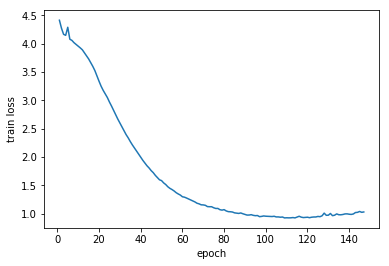
\includegraphics[scale=0.6]{pics/loss_optimal.png}}
\caption{Loss of 3-layer LSTM Optimized Model}
\label{fig1}
\end{figure}

\item Three LSTM Layers with different dimensionality:  

Dimensions in 3 LSTM: (512,512,256)

See loss figures in Fig.~\ref{fig2}.

\begin{figure}[htbp]
\centerline{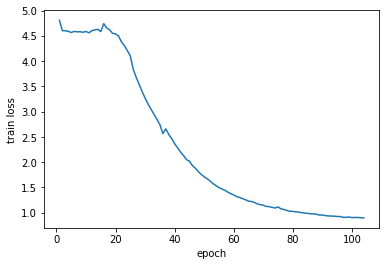
\includegraphics[scale=0.6]{pics/log_to256.png}}
\caption{Loss of 3-layer LSTM model with Modified Dimensions}
\label{fig2}
\end{figure}

\item Four LSTM Layers: Add one additional hidden LSTM layer as the fourth LSTM layer. 

Dimensions in 4 LSTM: (512,512,512,512)

See loss figures in Fig.~\ref{fig3}.
\end{itemize}

\begin{figure}[htbp]
\centerline{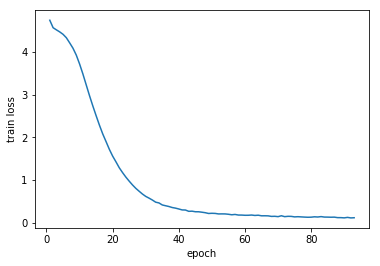
\includegraphics[scale=0.6]{pics/log_4lstm.png}}
\caption{Loss of 4-layer LSTM Optimized Model}
\label{fig3}
\end{figure}


It takes 20 hours to run 200 epochs with a 1080ti GPU.

After about 190 epochs, the model fits best.
In order to compare the training effects with different epochs, we generated several midi files with 1, 50, 100, 152, 191 epochs separately. See comparing figures in Fig.~\ref{fig4}.

\begin{figure}[htbp]
\centerline{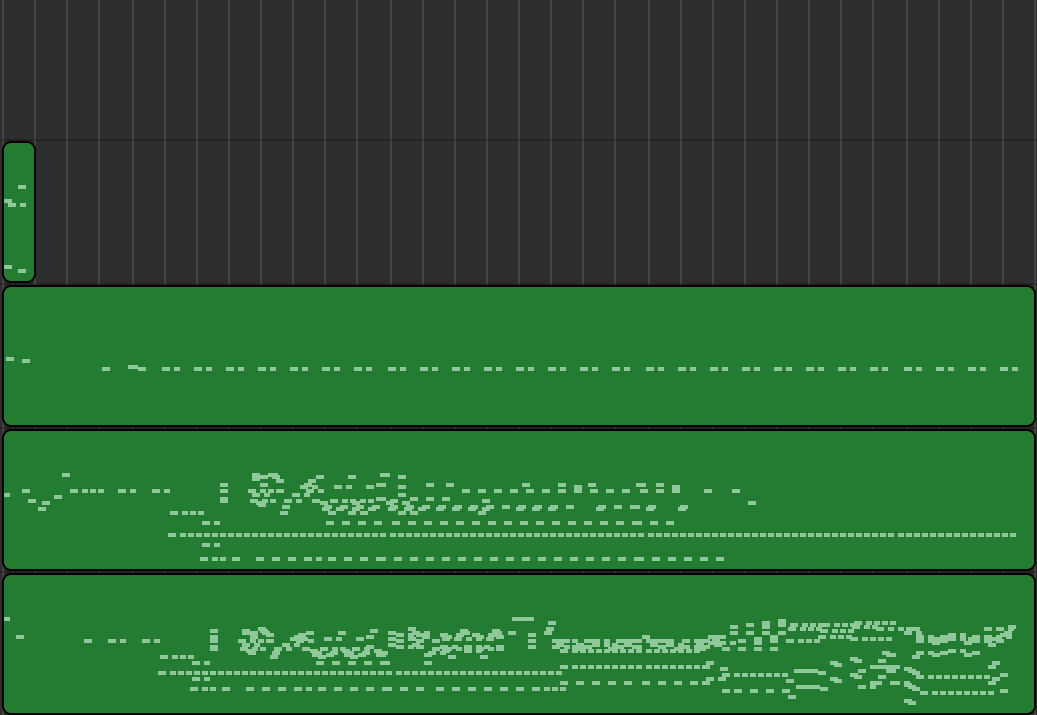
\includegraphics[scale=0.45]{compare_results.png}}
\caption{Comparison results with different epochs\protect\footnotemark}
\label{fig4}
\end{figure}
\footnotetext{from top to bottom are test samples with 1, 50, 100, 152, 191 epochs separately}

We believe that the same 100 previous beat pieces cannot guarantee that the following keys are unique, so we don't use accuracy as the measure. Instead, we let people to listen to our generated music and music from some related work and vote for the best music. See results in Table.~\ref{tab1}.

\begin{table}[htbp]
\caption{Voting Results}
\begin{center}
\begin{tabular}{|c|c|}
\hline
Program Name& Number of Votes\\
\hline
AI Jukebox& 7\\
Classical Piano Composer& 7\\
Deep jazz& 5\\
Deep Jammer& 4\\
\textbf{The Piano Boy}& 18\\
\hline
\end{tabular}
\label{tab1}
\end{center}
\end{table}

\section{Discussion of Results}
Our final model can predict rest note which has all 0s output and also any combination of note and chord which yields output that can have multiple 1s. Based on generated music, we realize that sometimes it seems like our model can memorize the training music, which is really amazing.

\section{Conclusions}
To improve the quality of generated music, we tried several different model structures, such as a three-LSTM-layer model with different dimensionality and a four-LSTM-layer model.

We also tried to use different beat lengths as input like using 40 instead of 100. However, the resulting outputs were not good.

Our final model is simply superior to the other experiments mentioned above. Of course, it is also better than some other similar applications chosen as our project baselines based on the survey result.

Now our model's prediction result is fixed if the input is determined, but we believe that music composition should be vibrant which means that same input could lead to different output. So we think that a probabilistic neural network model could be used in future work.

\begin{thebibliography}{00}
\bibitem{b1} McMahon, B. \textit{Music generator utilizing a Bidirectional LSTM architecture in Keras,} \url{https://github.com/cipher813/AI_Jukebox}.
\bibitem{b2} Sigurgeirsson, S. \textit{Classical Piano Composer,} \url{https://github.com/Skuldur/Classical-Piano-Composer}.
\bibitem{b3} Justin Svegliato and Sam Witty, \textit{Deep Jammer: A Music Generation Model}.
\bibitem{b4} Kim, J. \textit{Deep learning driven jazz generation using Keras \& Theano!,} \url{https://github.com/jisungk/deepjazz}.
\bibitem{b5} Ian Goodfellow, Yoshua Bengio, Aaron Courville. Deep Learning[M]. MIT Press, 2016.
\bibitem{b6} M.S. Cuthbert and C. Ariza. music21: A toolkit for computer-aided musicology and symbolic music data. In \textit{9th International Society for Music Information Retrieval Conference}, pages 637-642, Utrecht, Netherlands, August 2010.
\end{thebibliography}
\vspace{12pt}


\end{document}
